\section{Testing}


\subsection{NAND}

\subsection{NOR2}

\subsection{XOR2}

\subsection{DFF}

Figure \ref{fig:DFFTestSchem} shows the test circuit used to test the DFF.The vpulse elements allow generation of a clock and an alternating D signal using correct timing and phase. By connecting the Q of the first gate to that of the second it also is useful for demonstrating the required fanout of 1. By choosing suitable values for CLK D and load capacitance a variety of situations can be simulated.

\begin{figure}[h]  
\centering
   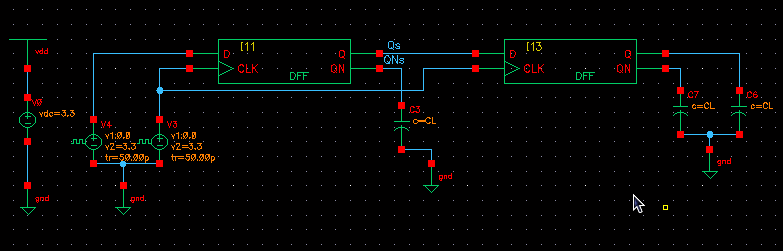
\includegraphics[width=0.45\textwidth]{Figures/DFFTestSchem.png}
\caption{DFF Test Circuit Schematic.}
\label {fig:DFFTestSchem}
\end{figure}

Figure \ref{fig:DFFTestFunc} shows the output of a simulation using the above circuit. The load is set to 320 fF to represent a relatively high load case. As is shown the output Q does not change until the positive clock edge and holds its data until subsequent positive edges. The input D also propagates correctly through both flip flops.

\begin{figure}[h]  
\centering
   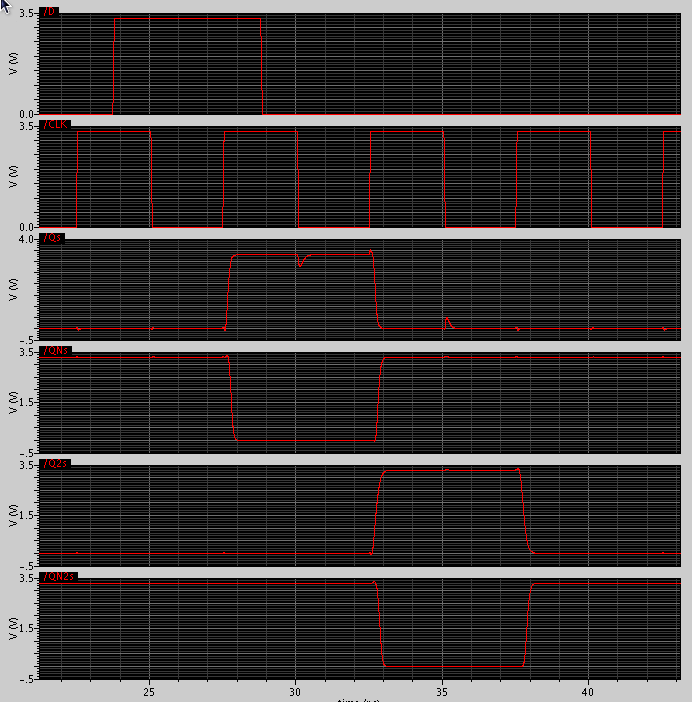
\includegraphics[width=0.45\textwidth]{Figures/DFFTestFunc.png}
\caption{DFF Functionality Test.}
\label {fig:DFFTestFunc}
\end{figure}

SPEED TESTING

Figure \ref{fig:DFFTestSpeed} shows a zoomed in section of the output of the simulation. This shows a Q rise time of 0.21 ns and a fall time of 0.22 ns which for a 320pF load is quite fast. However the design does suffer slightly from its large transistors which although deliver good rise time the propagation delay is 0.36 ns.

\begin{figure}[h]  
\centering
   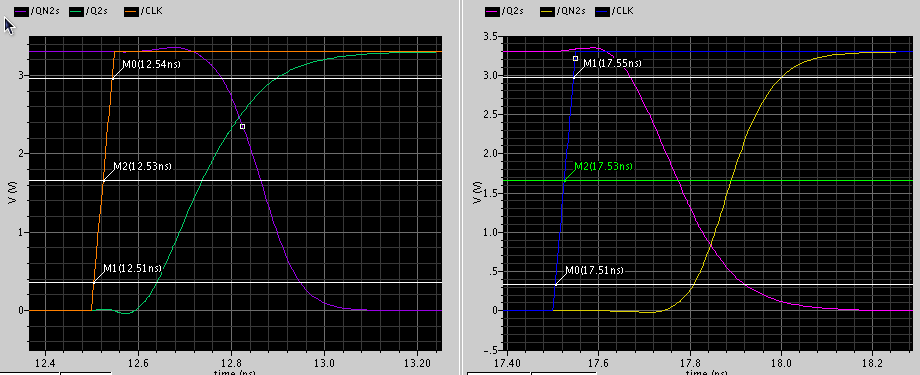
\includegraphics[width=0.45\textwidth]{Figures/DFFTestSpeed.png}
\caption{DFF Speed Test.}
\label {fig:DFFTestSpeed}
\end{figure}

The disruption in the Q signal connected to the input of the second gate when the clock pulses as seen at 30ns in figure \ref{fig:DFFTestFunc} is caused by the transmission gates switching on the clock edge and latching the data for the usbsequent edge. As this is below the threshold of 10 percent it should not cause any problems as part of a asynchronous or synchronous design.


\subsection{Dual Edge Triggered Flip Flop}

Figure \ref{fig:DETFFTestSchem} shows the test circuit used to test the DFF.The vpulse elements allow generation of a clock and an alternating D signal using correct timing and phase. By connecting the Q of the first gate to that of the second it also is useful for demonstrating the required fanout of 1. By choosing suitable values for CLK D and load capacitance a variety of situations can be simulated.

\begin{figure}[h]  
\centering
   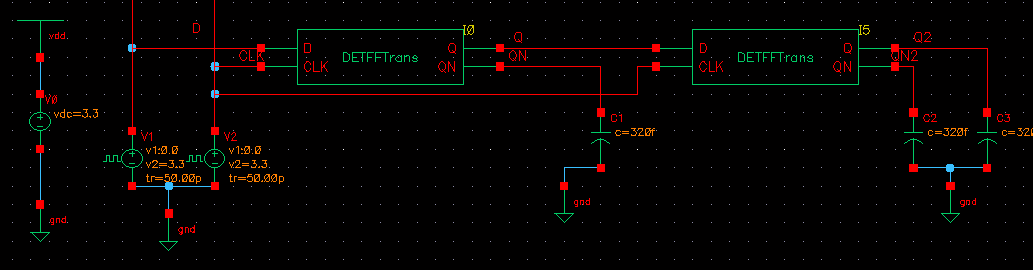
\includegraphics[width=0.45\textwidth]{Figures/DETFFTestSchem.png}
\caption{DETFF Test Circuit Schematic.}
\label {fig:DETFFTestSchem}
\end{figure}

Figure \ref{fig:DETFFTestFunc} shows the output of a simulation using the above circuit. The load is set to 320 fF to represent a relatively high load case. As is shown the output Q does not change until the positive clock edge and holds its data until subsequent clock edges. The input D also propagates correctly through both flip flops.

\begin{figure}[h]  
\centering
   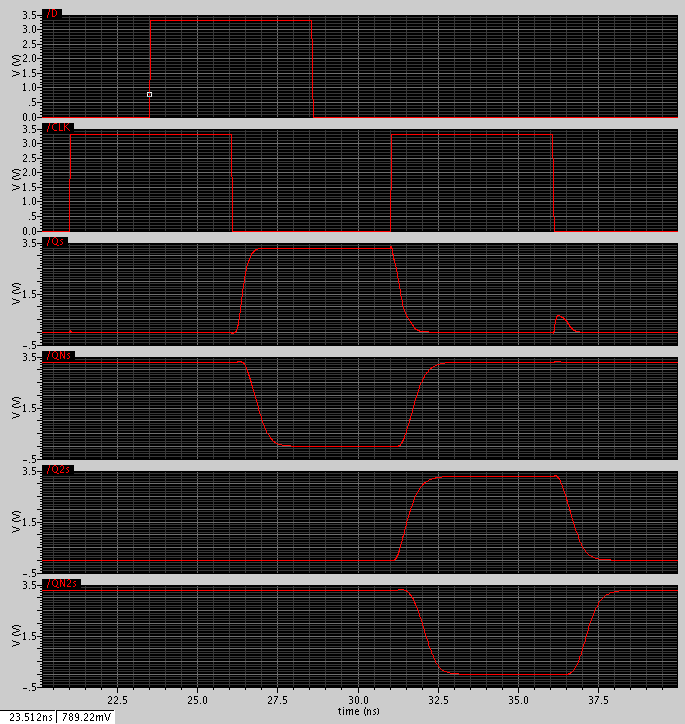
\includegraphics[width=0.45\textwidth]{Figures/DETFFTestFunc.png}
\caption{DETFF Functionality Test.}
\label {fig:DETFFTestFunc}
\end{figure}

Figure \ref{fig:DETFFTestSpeed} shows a zoomed in section of the output of the simulation. This shows a Q rise time of 0.8 ns and a fall time of 0.65 ns which for a 320pF load is reasonable for this gate. The disparity between the times suggest a different PMOS/Nmos ratio could be beneficial.

\begin{figure}[h]  
\centering
   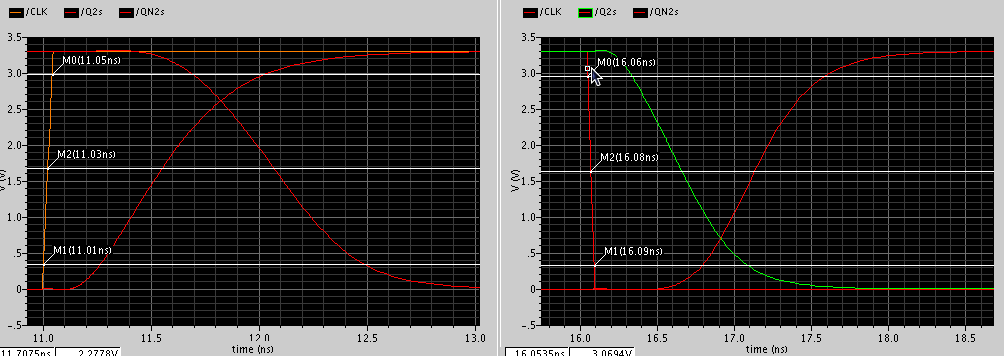
\includegraphics[width=0.45\textwidth]{Figures/DETFFTestSpeed.png}
\caption{DETFF Speed Test.}
\label {fig:DETFFTestSpeed}
\end{figure}

The disruption in the Q signal connected to the input of the second gate when the clock pulses as seen at 30ns in figure \ref{fig:DFFTestFunc} is caused by the transmission gates switching on the clock edge and latching the data for the subsequent edge. As this is below the threshold of 10 percent it should not cause any problems as part of a asynchronous or synchronous design.


\subsection{C Element}

\subsection{Dual Rail AND}

Figure \ref{fig:DualRailANDTestSchem} shows the test circuit for the Dual Rail AND (DRAND) there are 2 clocks for data generation one set at half the frequency of the other allowing for all 4 data states to be modelled. The outpus of the clocks are connected to the A/B 1 connections and also go through an inverter to create the relevant A/B 0 signal. The third clock is used in conjunction with the AND structure to add the '00' spacer state to reset the C Elements between data.

\begin{figure}[h]  
\centering
   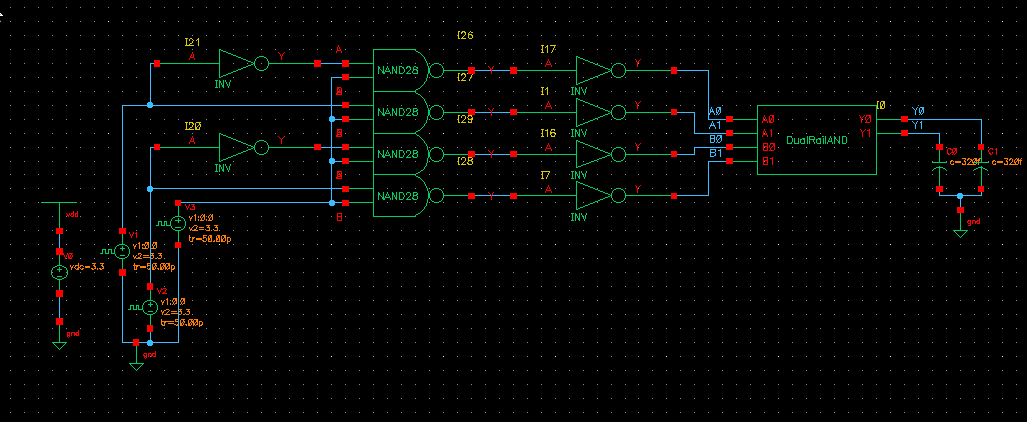
\includegraphics[width=0.45\textwidth]{Figures/DualRailANDTestSchem.png}
\caption{Dual Rail AND Test Schematic.}
\label {fig:DualRailANDTestSchem}
\end{figure}

Figure \ref{fig:DualAndCorrectOperation} shows the output of a simulation using the above circuit. As you can see this the output Y0 goes low and Y1  goes high only when both A1 and B1 are asserted it also correctly transmits the '00' spacer behaviour.

\begin{figure}[h]  
\centering
   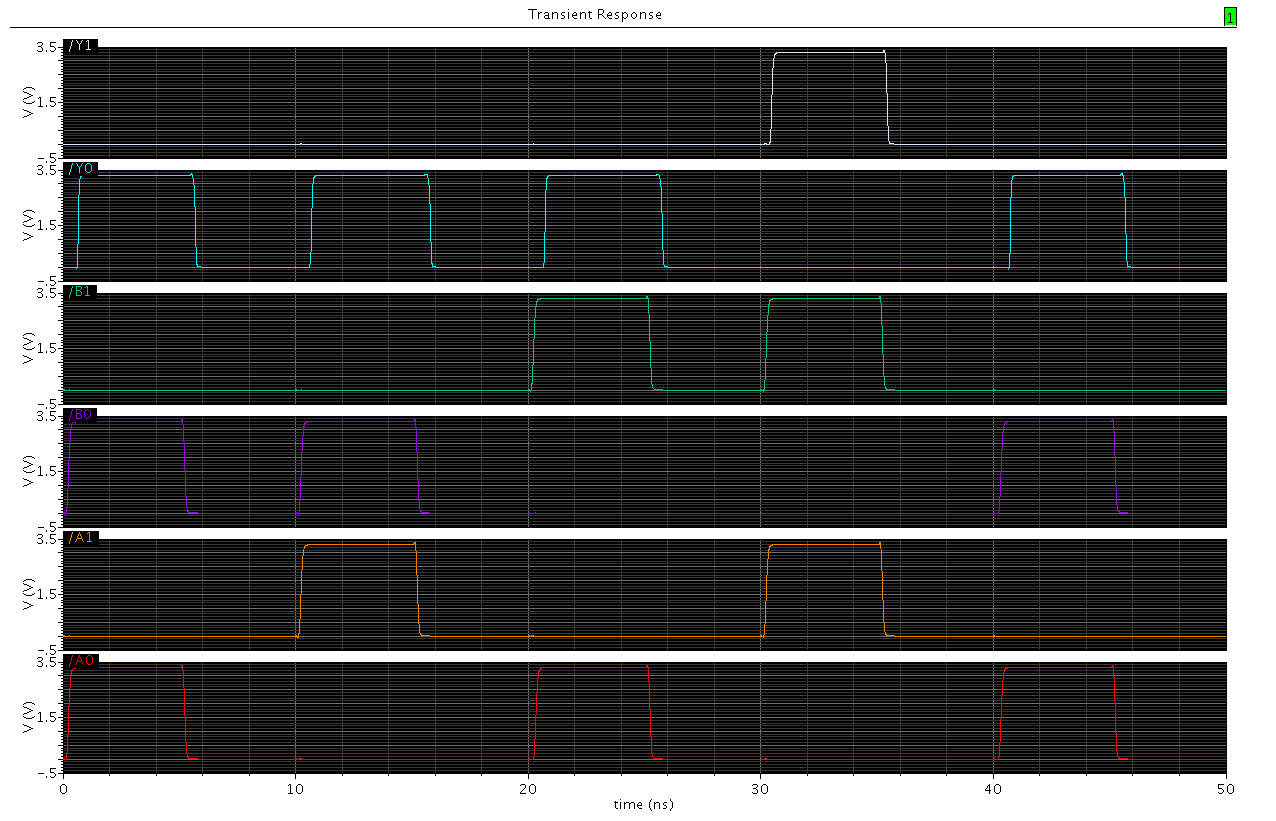
\includegraphics[width=0.45\textwidth]{Figures/DualAndCorrectOperation.png}
\caption{Dual Rail AND Simulation showing correct operation.}
\label {fig:DualAndCorrectOperation}
\end{figure}









\subsection{1-bit Subtractor}

\subsection{2-to-1 Multiplexor}

\subsection{Mutex Element}

TEST CIRCUIT
FUNCTIONALITY TESTING 
SPEED TESTING
LAYOUT VS SCHEMATIC 
ERRONIOUS BEHAVIOUR